\chapter{EEDURO-Delta-Roboter}
In diesem Kapitel wird das zweite Fallbeispiel mit dem EEDURO-Delta-Roboter (Abbildung \ref{Ab:eeduro}) vorgestellt.
Der EEDURO-Delta ist ein kleiner Delta-Roboter, der für Schulungszwecke gedacht ist.
Die Modell-Beschreibung des Roboters ist im \textit{URDF}"=Format gehalten.
Dabei wurde gleich vorgegangen wie für die Motor"=Apparatur\footnote{siehe Kapitel \ref{chap:motor}}, deshalb werden in diesem Kapitel nur noch neue Aspekte erläutert.
\begin{figure}[ht!]
	\centering
	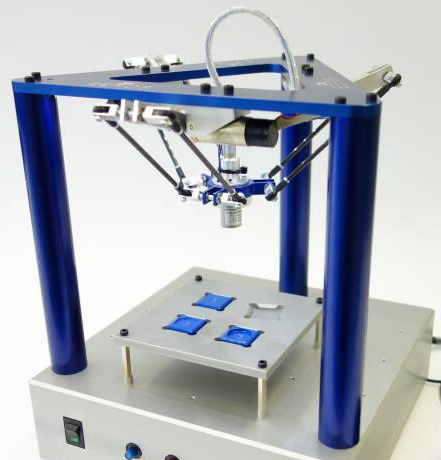
\includegraphics[width=7cm]{images/eeduro_delta.png}
	\caption{EEDURO-Delta \cite{eeduro}}
	\label{Ab:eeduro}
\end{figure}

\section{Modell}
\label{chap:delta-modell}
Die Modell"=Beschreibung des Deltaroboters wurde im \textit{URDF}"=Format erstellt.
Die ganze Datei ist im Repository \textit{\textit{"}eeduro\_delta\textit{"}}~\footnote{\url{https://github.com/manuelilg/eeduro_delta/tree/master/eeduro_delta_description/urdf}} abgelegt.
Speziell ist aber das zusätzlich noch die Skriptsprache \textit{XACRO}\footnote{siehe Kapitel \ref{chap:xacro}} beim erstellen der \textit{URDF}"=Datei eingesetzt wurde.

%Das Modell des Delta-Roboter kann grob in drei gleiche Teile aufgeteilt werden:
%\begin{itemize}
%\item Rahmen (base)
%\item Arm (arm 1-3)
%\item Werkzeug (tool)
%\end{itemize}
%
%Der Arm selber besteht aus einem Oberarm auch Link 1 genannt und aus einem Unterarm.
%Der Unterarm selber besteht selber wieder aus:
%\begin{itemize}
%\item Doppelgabel (Link 2)
%\item zwei Stangen (Link 3.1 und Link 3.2)
%\item 2.Doppelgabel (Link 4)
%\end{itemize}

Die Benennung der unterschiedlichen Teile ist in Abbildung \ref{Ab:delta-schematisch} aufgezeigt.

\begin{figure}[ht!]
	\centering
	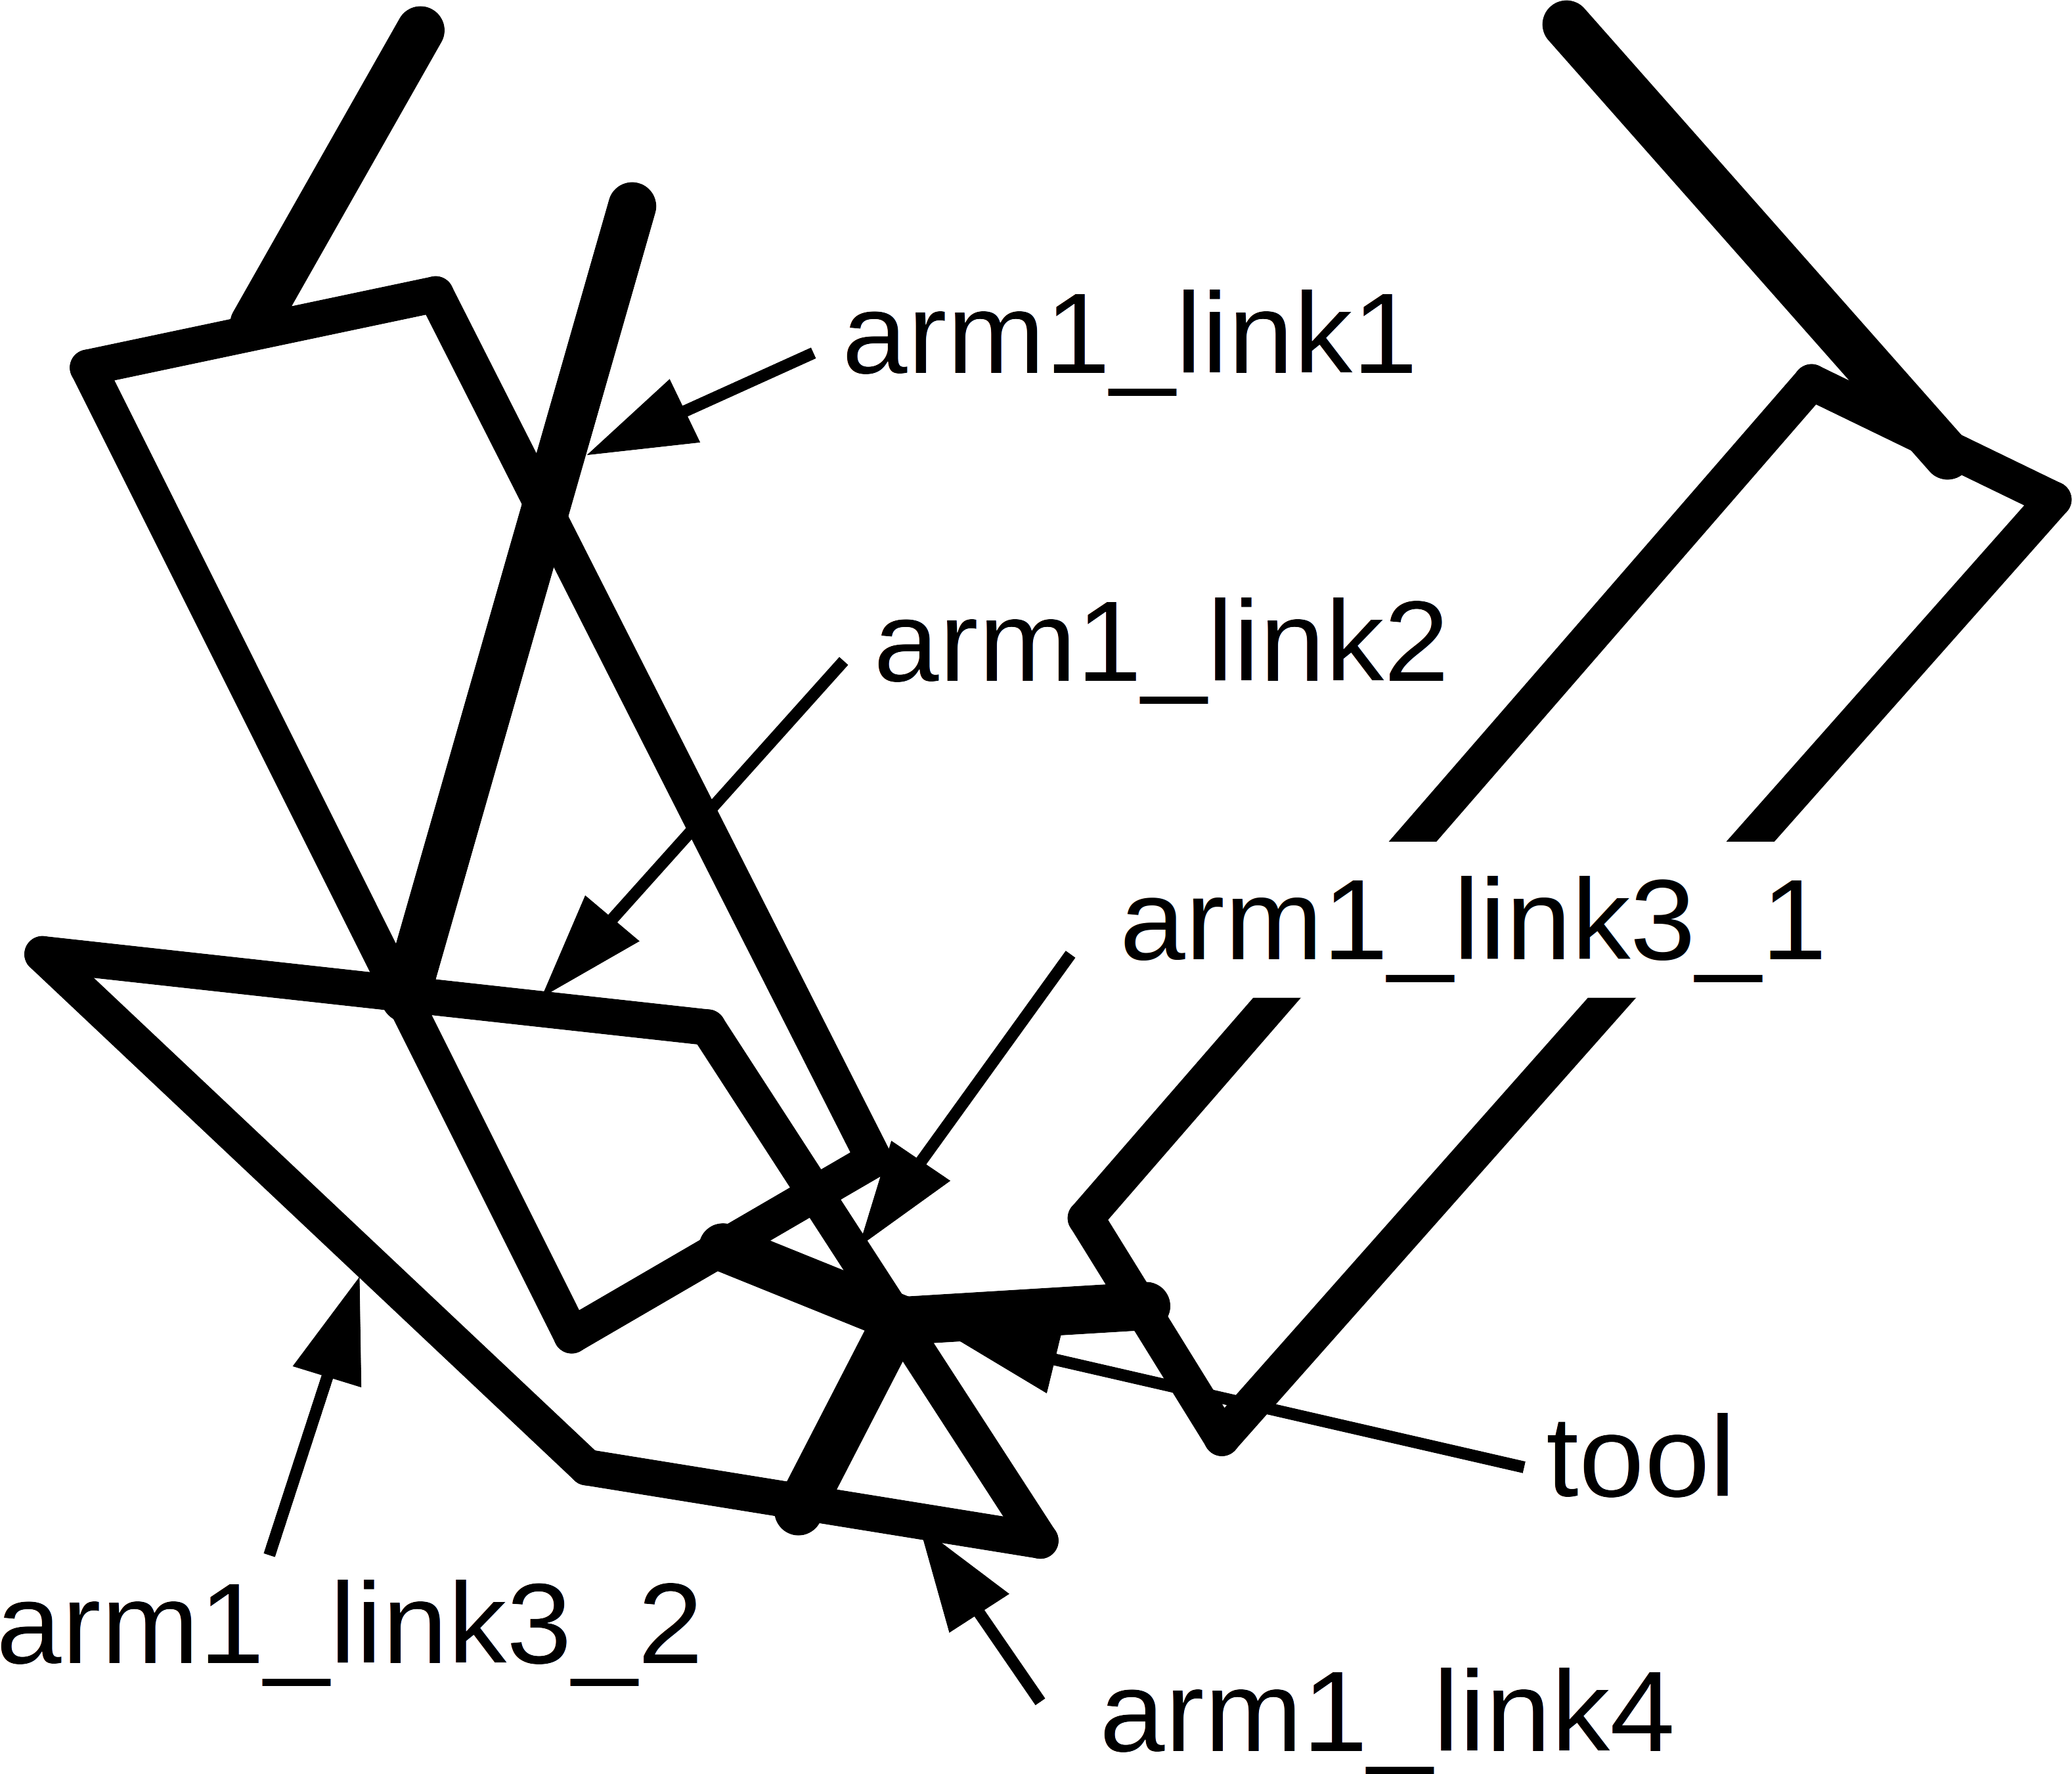
\includegraphics[width=6cm]{images/delta.png}
	\caption{Schematische Darstellung Delta-Roboter}
	\label{Ab:delta-schematisch}
\end{figure}

Wie beim Motor muss die kinematisch Kette geschlossen werden mit dem \textit{SDF}"=Joint Element (dargestellt in Abbildung \ref{Ab:delta-struktur} mit grünen Ellipsen).

\begin{figure}[ht!]
	\centering
	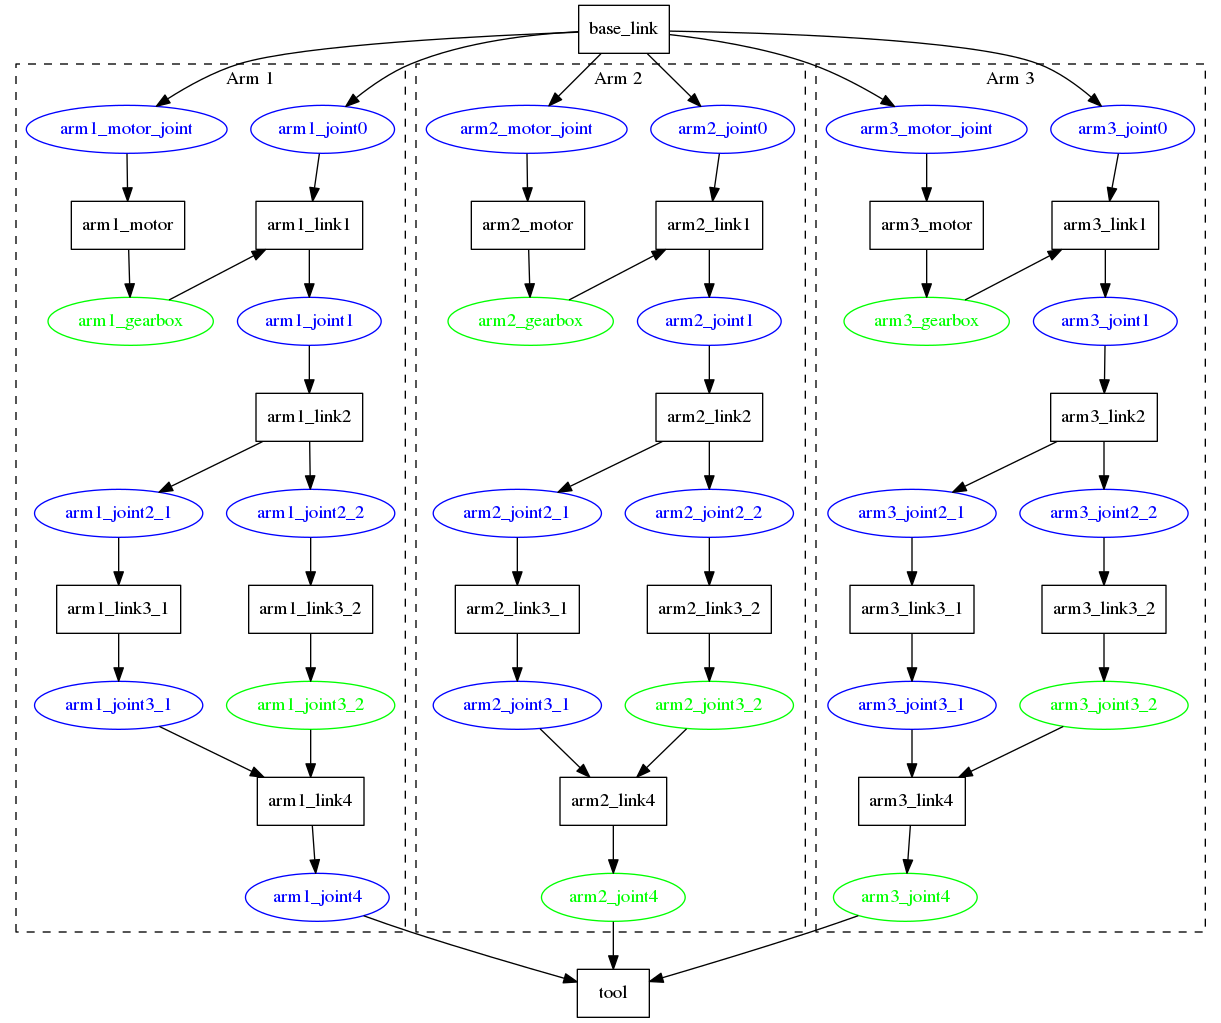
\includegraphics[width=14.5cm]{images/delta_struktur.png}
	\caption{kinematische Struktur EEDURO-Delta}
	\label{Ab:delta-struktur}
\end{figure}

\subsection{Parameter für Modell}
In diesem Abschnitt wird darauf eingegangen, welche Parameter es braucht für die Erstellung vom Modell.
\begin{itemize}
\item Masse und Trägheitstensor von allen Links
\item Längenmasse wie Abstand zwischen zwei Gelenken
\item Geometrie von allen Links
\end{itemize}

Ein Teil dieser Parameter konnten aus Datenblättern gewonnen werden.
Diese Datenblätter sind im Repository \textit{\textit{"}eeduro\_delta\textbf{"}}~\footnote{\url{https://github.com/manuelilg/eeduro\_delta/tree/master/eeduro\_delta\_description/datasheets}} zu finden.

\subsubsection{Berechnung Masse und Trägheitstensor}
Für jedes Glied musste die Masse und Rotationsträgheit berechnet werden, damit das Modell des Roboters sich in der Simulation wie der reale Roboter verhält.
Die Glieder bestehen jedoch aus mehreren Bauteilen.
Dieser Umstand verkompliziert die Berechnung sehr.
Auch erschwerend kam hinzu, dass die CAD"=Daten nur im \textit{STEP}"=Austauschformat vorliegend waren.

Das führt zu folgendem Arbeitsablauf:
\begin{enumerate}
\item für jedes Glied/Baugruppe: 
\begin{enumerate}
\item eine CAD"=Datei erstellen
\item für jedes Bauteil in Baugruppe folgende Daten exportieren
\begin{enumerate}
\item Volumen von Körper
\item Schwerpunkt von Körper
\item Rotationsträgheit"=Tensor von Volumen
\end{enumerate}
\item exportierte Daten in Matlab eintragen
\item für jedes Bauteil Dichte in Matlab hinterlegen
\item für jedes Bauteil mit Dichte: Masse und Rotationsträgheit ausrechnen  
\end{enumerate}
\item Schwerpunkt und Masse von Baugruppe bestimmen
\item Rotationsträgheit von Baugruppe ausrechnen (Steinerscher Satz für jedes Bauteil anwenden)
\end{enumerate}

Die CAD"=Daten und Matlab"=Dateien sind im Repository \textit{\textit{"}eeduro\_delta\textit{"}}~\footnote{\url{https://github.com/manuelilg/eeduro_delta/tree/master/eeduro_delta_description}} zufinden.

\subsubsection{XACRO}
\label{chap:xacro}
\textit{XACRO}~\footnote{\url{http://wiki.ros.org/xacro}} ist eine Makro Sprache für XML"=Dateien.
Mit \textit{XACRO} können kürzere und einfacher zu unterhaltende XML"=Dateien erstellt werden.
Denn mit Hilfe der Makros können Wiederholungen vermieden werden.
Auch kann Dank \textit{XACRO} eine XML"=Datei in mehrere Unterdateien aufgeteilt werden.
Somit kann ein komplexes System logisch in Untersysteme aufgeteilt werden, die dann jeweils in einer eigenen XML"=Datei beschrieben werden. 



\section{EEDURO-Delta Joint State Publisher}
Der \textit{ROS}"=Knoten \textit{\textit{"}eeduro\_delta\_joint\_state\_publisher\textit{"}} erfüllt folgende Aufgaben:
\begin{itemize}
\item Direkt"=Kinematik berechnen
\item alle Gelenkwinkel ausrechnen
\end{itemize}
Die Direkt"=Kinematik berechnet die Werkzeug"=Position aus den drei Gelenkwinkeln von den Oberarmen des Delta"=Roboters.
Mit Werkzeug"=Position können anschliessend die Winkel aller Gelenke des Roboters berechnet werden.
Somit müssen für die visualisiert des EEDURO"=Delta"=Roboters im \textit{RViz} nur die drei Gelenkwinkel von den Oberarmen bekannt sein.
Diese Winkel können wahlweise von der Hardware oder von der Simulation kommen.

Eine Ausführliche Dokumentation dieses \textit{ROS}"=Knotens kann im Anhang xx gefunden werden. %TODO anhang

In Abbildung \ref{Ab:prozess} ist der ganze Prozess"=Graph mit allen beteiligten Komponenten dargestellt.

\begin{figure}[ht!]
	\centering
\begin{tikzpicture}[scale=1,node distance=5mm,
	link/.style={rectangle, draw=black, thick, inner sep=7},
	joint/.style={ellipse, draw=blue, thick},
	>=latex]
 	
 \node[link] (pub1) {eeduro\_delta\_joint\_state\_publisher};
 \node[link, above left=of pub1] (hard) {hardware};
 \node[link, above right=of pub1] (sim) {simulation};
 \node[link, below=of pub1] (pub2) {joint\_state\_publisher};
 \node[link, below=of pub2] (pub3) {robot\_state\_publisher};
 \node[link, below=of pub3] (rviz) {RViz};
 
 \path[->, thick]
 	(hard) edge (pub1)
 	(sim) edge (pub1)
 	(pub1) edge (pub2)
 	(pub2) edge (pub3)
 	(pub3) edge (rviz);
 	
\end{tikzpicture}
	\caption{Prozess-Graph Visualisierung Deltaroboter}
	\label{Ab:prozess}
\end{figure}

\section{Installation}
In diesem Abschnitt wird die Installation des Repository \textit{\textit{"}eeduro\_delta\textbf{"}} gezeigt.

Alle erforderliche Repositorys in \textit{Workspace} klonen:
\begin{lstlisting}
$ cd ~/catkin_ws/src
$ git clone https://github.com/manuelilg/eeduro_delta.git
$ git clone https://github.com/manuelilg/gazebo_ros_joint_force.git
$ git clone https://github.com/manuelilg/gazebo_ros_pkgs.git
\end{lstlisting} 

Alle geklonten Packages kompilieren:
\begin{itemize}
\item mit \textit{catkin-tools}~\footnote{\url{http://catkin-tools.readthedocs.io/en/latest/index.html}} (empfohlen)
\begin{lstlisting}
$ catkin build
\end{lstlisting}
\item mit \textit{catkin\_make}~\footnote{\url{http://wiki.ros.org/catkin/commands/catkin\_make}}
\begin{lstlisting}
$ catkin_make
\end{lstlisting}
\end{itemize}

Umgebungsvariablen laden für Ausführung:
\begin{lstlisting}
$ source ~/catkin_ws/devel/setup.bash
\end{lstlisting}

\section{Ausführen}
In diesem Abschnitt wird gezeigt wie die verschiedenen Bestandteile gestartet werden können.
\subsection{Gazebo}
\textit{Gazebo}"=Simulation von EEDURO"=Delta starten (Simulation ist pausiert)
\begin{lstlisting}
$ roslaunch eeduro_delta_gazebo eeduro_delta_world.launch
\end{lstlisting}

\subsection{Gazebo mit RViz}
\textit{Gazebo} zusammen mit \textit{RViz} starten (vgl. Abbildung \ref{Ab:prozess})
\begin{lstlisting}
$ roslaunch eeduro_delta_gazebo eeduro_delta_rviz.launch
\end{lstlisting}


\section{RQt}
\textit{RQt} für das Ploten der System"=Grössen starten
\begin{lstlisting}
$ roslaunch 
\end{lstlisting}
